\documentclass[journal, a4paper]{IEEEtran}

% some very useful LaTeX packages include:

%\usepackage{cite}      % Written by Donald Arseneau
                        % V1.6 and later of IEEEtran pre-defines the format
                        % of the cite.sty package \cite{} output to follow
                        % that of IEEE. Loading the cite package will
                        % result in citation numbers being automatically
                        % sorted and properly "ranged". i.e.,
                        % [1], [9], [2], [7], [5], [6]
                        % (without using cite.sty)
                        % will become:
                        % [1], [2], [5]--[7], [9] (using cite.sty)
                        % cite.sty's \cite will automatically add leading
                        % space, if needed. Use cite.sty's noadjust option
                        % (cite.sty V3.8 and later) if you want to turn this
                        % off. cite.sty is already installed on most LaTeX
                        % systems. The latest version can be obtained at:
                        % http://www.ctan.org/tex-archive/macros/latex/contrib/supported/cite/

\usepackage{graphicx}   % Written by David Carlisle and Sebastian Rahtz
                        % Required if you want graphics, photos, etc.
                        % graphicx.sty is already installed on most LaTeX
                        % systems. The latest version and documentation can
                        % be obtained at:
                        % http://www.ctan.org/tex-archive/macros/latex/required/graphics/
\usepackage{subfig}
                        % Another good source of documentation is "Using
                        % Imported Graphics in LaTeX2e" by Keith Reckdahl
                        % which can be found as esplatex.ps and epslatex.pdf
                        % at: http://www.ctan.org/tex-archive/info/

%\usepackage{psfrag}    % Written by Craig Barratt, Michael C. Grant,
                        % and David Carlisle
                        % This package allows you to substitute LaTeX
                        % commands for text in imported EPS graphic files.
                        % In this way, LaTeX symbols can be placed into
                        % graphics that have been generated by other
                        % applications. You must use latex->dvips->ps2pdf
                        % workflow (not direct pdf output from pdflatex) if
                        % you wish to use this capability because it works
                        % via some PostScript tricks. Alternatively, the
                        % graphics could be processed as separate files via
                        % psfrag and dvips, then converted to PDF for
                        % inclusion in the main file which uses pdflatex.
                        % Docs are in "The PSfrag System" by Michael C. Grant
                        % and David Carlisle. There is also some information
                        % about using psfrag in "Using Imported Graphics in
                        % LaTeX2e" by Keith Reckdahl which documents the
                        % graphicx package (see above). The psfrag package
                        % and documentation can be obtained at:
                        % http://www.ctan.org/tex-archive/macros/latex/contrib/supported/psfrag/

%\usepackage{subfigure} % Written by Steven Douglas Cochran
                        % This package makes it easy to put subfigures
                        % in your figures. i.e., "figure 1a and 1b"
                        % Docs are in "Using Imported Graphics in LaTeX2e"
                        % by Keith Reckdahl which also documents the graphicx
                        % package (see above). subfigure.sty is already
                        % installed on most LaTeX systems. The latest version
                        % and documentation can be obtained at:
                        % http://www.ctan.org/tex-archive/macros/latex/contrib/supported/subfigure/

\usepackage{url}        % Written by Donald Arseneau
                        % Provides better support for handling and breaking
                        % URLs. url.sty is already installed on most LaTeX
                        % systems. The latest version can be obtained at:
                        % http://www.ctan.org/tex-archive/macros/latex/contrib/other/misc/
                        % Read the url.sty source comments for usage information.

%\usepackage{stfloats}  % Written by Sigitas Tolusis
                        % Gives LaTeX2e the ability to do double column
                        % floats at the bottom of the page as well as the top.
                        % (e.g., "\begin{figure*}[!b]" is not normally
                        % possible in LaTeX2e). This is an invasive package
                        % which rewrites many portions of the LaTeX2e output
                        % routines. It may not work with other packages that
                        % modify the LaTeX2e output routine and/or with other
                        % versions of LaTeX. The latest version and
                        % documentation can be obtained at:
                        % http://www.ctan.org/tex-archive/macros/latex/contrib/supported/sttools/
                        % Documentation is contained in the stfloats.sty
                        % comments as well as in the presfull.pdf file.
                        % Do not use the stfloats baselinefloat ability as
                        % IEEE does not allow \baselineskip to stretch.
                        % Authors submitting work to the IEEE should note
                        % that IEEE rarely uses double column equations and
                        % that authors should try to avoid such use.
                        % Do not be tempted to use the cuted.sty or
                        % midfloat.sty package (by the same author) as IEEE
                        % does not format its papers in such ways.

\usepackage{amsmath}    % From the American Mathematical Society
                        % A popular package that provides many helpful commands
                        % for dealing with mathematics. Note that the AMSmath
                        % package sets \interdisplaylinepenalty to 10000 thus
                        % preventing page breaks from occurring within multiline
                        % equations. Use:
%\interdisplaylinepenalty=2500
                        % after loading amsmath to restore such page breaks
                        % as IEEEtran.cls normally does. amsmath.sty is already
                        % installed on most LaTeX systems. The latest version
                        % and documentation can be obtained at:
                        % http://www.ctan.org/tex-archive/macros/latex/required/amslatex/math/
\usepackage{amssymb}


% Other popular packages for formatting tables and equations include:

%\usepackage{array}
% Frank Mittelbach's and David Carlisle's array.sty which improves the
% LaTeX2e array and tabular environments to provide better appearances and
% additional user controls. array.sty is already installed on most systems.
% The latest version and documentation can be obtained at:
% http://www.ctan.org/tex-archive/macros/latex/required/tools/

% V1.6 of IEEEtran contains the IEEEeqnarray family of commands that can
% be used to generate multiline equations as well as matrices, tables, etc.

% Also of notable interest:
% Scott Pakin's eqparbox package for creating (automatically sized) equal
% width boxes. Available:
% http://www.ctan.org/tex-archive/macros/latex/contrib/supported/eqparbox/

% *** Do not adjust lengths that control margins, column widths, etc. ***
% *** Do not use packages that alter fonts (such as pslatex).         ***
% There should be no need to do such things with IEEEtran.cls V1.6 and later.

%Start: Das hier sorgt dafür, dass Umlaute funktionieren.
%\usepackage[main=ngerman, english]{babel}
\usepackage[main=ngerman, english]{babel}
\usepackage[utf8]{inputenc}
\usepackage{algorithm}
\usepackage{algorithmic}
\usepackage{amsmath}
\usepackage{gensymb}
%Ende: Das hier sorgt dafür, dass Umlaute funktionieren.
%\theoremstyle{theorem}
\newtheorem{theorem}{Theorem}[section]

% Your document starts here!
\begin{document}
	\selectlanguage{english}
	% Define document title and author
	\title{Waddle -- Waddington's epigentic landscape}
	\author{Felicia Burtscher}
	\thanks{Special thanks go to Michael PH Stumpf, Suhail A Islam, Rowan Brackston, Ivan Croydon Veleslavov and the whole Julia community out there.}\\
	
\markboth{Imperial College: MSc Bioinformatics and Theoretical Systems Biology, \today}{}
\maketitle
%%%%%%
%WHAT I DID:
%1. literature research -- set alerts on pubmed, twitter and google search
%2. create refWorks -- for bibtex bibliograhy later
%%%%%%


% Write abstract here
\begin{abstract}
The \textit{Waddington} or \textit{epigenetic landscape} concept has become an important framework to reason about developmental processes. This project develops a set of Julia tools to determine the structure of such landscapes for a given dynamical system, as well as single cell data. We implement the probability flux method (PFM) of constructing a landscape, additionally applying kernel density estimation (KDE). Stability analysis is conducted on dynamical systems and their corresponding landscapes. In conjunction to that a second, more accurate approach %REALLY??
of the landscape is performed: Minimal Action Path (MAP) method. The latter one has a direct interpretation to the force that would need to be applied to cross the landscape between two chosen points. Due to computational complexity, we limited our approach to only simulate the quasipotential given two points in space. %% IS THAT STILL TRUE?
For high dimensional systems, the topic of dimensionality reduction is addressed, with corresponding tools developed to aid visualisation of these high dimensional systems. 
Reasonable results could be yield for the 2-dimensional KDE as well as the PFM on the CPU; the PFM on the GPU posed a real challenge due to problems outlined in the group report and is still in progress.


%SET SCIENTIFIC CONTEXT
%METHODS, RESULTS, CONCLUSIONS CLEAR AND PRECISE
\end{abstract}

\section{Preface}
The following report will focus on different methods of dimensionality reduction and literature research as this was my main focus during the project. 
% The theory can be found in the group report
% also time on Bayesian Gaussian Latent variabel model and Hopfland, discovered together with MH
Other parts I contributed to was the Genetic Algorithm (GA) to approximate the MAP, converting the MAP between two points into a quasi-potential, implementing different kernel methods for the kernel density estimation (KDE) as well as different information theory approaches to the given sample data set. However, this will not be the subject of the following report to avoid overlap with the other reports and due to the restrictive word count. For an overview we refer to the group project report, for the information theory approaches we refer to Madeleine Hall's report, for the GA we refer to Lucas Ducrot's report. The final code can be found on \begin{verbatim}
https://github.com/burfel/waddington-project.
\end{verbatim}	
The \textit{README.md} was kept self-explanatory and should give an overview of the main tools implemented. \\
Other important tasks of mine were documentation and commenting code, keeping our github repository nice and tidy and sharing links to interesting papers via a pad as literature research was a major part in the project. \\

It should be noted that in the following, I assume the reader to have read our group report. My following individual report is kept on a personal note and should reflect my main contributions to the research project, challenges I faced and especially learnings thereof. 


%TODO:
%INSERT ALL REFERENCES FROM THE PAD (MAINLY SECTION LITERATURE RESEARCH), GITHUB
	

%\tableofcontents 
% Each section begins with a \section{title} command

%\section{Task Description}
%
%Our data set consists of images of 20 characters of \textit{The Simpsons} with labels. The data originates from the Kaggle contest \textit{Simpsons by the Data}. There are 200 to 1500 examples per character offering an unbalanced data set. The images have different shapes and the characters are scattered throughout the images. Our goal is to develop an algorithm which given an input image containing a Simpson character is capable to classify, i.e. recognize the Simpsons character in the image correctly. In \textit{The Simpsons} data set this is the character the image shows. We are looking for a function that maps the input images to the labels of the images.
%\begin{figure}[!ht]
%	\centering
%  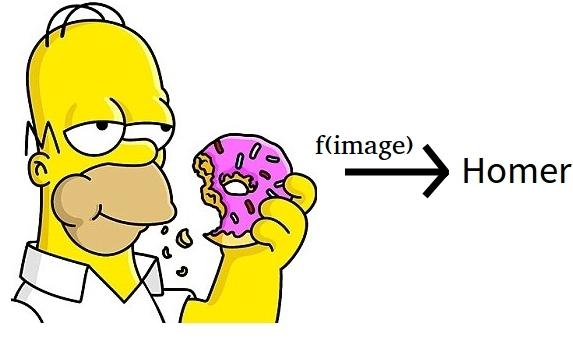
\includegraphics[width=0.3\textwidth]{Image3.jpeg}
%	\caption{Homer Simpson}
%	\label{Homer}
%\end{figure}

%%%%------------
%\section{Background, context and motivation}
%For the motivation
%
%%%------------
%\section{Mathematical framework}
%
%%%%----------
%\subsection{Probability flux method}
%%%%----------
%\subsection{Kernel density estimation}
%
%%%%----------
%\subsection{Stability analysis}
%
%%%------------
%\section{Dynamical systems}
%
%%%%----------
%\subsection{2-Dimensional model}
%
%%%%----------
%\subsection{Simulations}
%

%%------------

\section{Introduction}

EXPLAIN TOPIC CLEARLY, SEE REVIEW 

\section{Literature research}

START WITH SUBSTANTIAL BACKGROUND READING

EXPLAIN PREVIOUS WORK
AIMS, ADVANCES CLEARLY DEFINED

Before I started with anything (except some toy models) I did some extensive literature research on the work that has already been done regarding Waddington's landscape. This was necessary as there was no specific task given, and no underlying biological question that needed to be answered. It was probably one of the major challenges of the whole project: To find a (convincing) motivation of the project and to come up with a specific goal.
It is challenging to synthesise the work that has been done as very different approaches have been taken. In order to situate our work within the wider literature, I am going to highlight the major state-of-the-art methods that have been developed by other groups:

\subsection{Monocle}
\subsection{Topslam}
\subsection{Hopland}
TALK ABOUT BGLPVM here; too complicated/ involved approach that could not be achieved within the given time frame, but might be interesting to look into in the future --> MOVE TO OUTLOOK

For a more thorough review on the Hopland approach, we refer to Madeleine Hall's individual report.
\subsection{Hadoop}??
\subsection{Wishbone}?
\subsection{SCUBA}?

As so much has been done already, and we did not want to reinvent the wheel, we defined our goal as follow: To develop a set of tools and methods to simulate (via the Probability Flux Method (PFM), Kernel Density Estimation (KDE) and the Minimum-Action Path (MAP)) and analyse the given landscape including dynamical systems stability analysis; moreover, we want to provide the user with various methods to read in the data (including from sbml files), extract information from the given data set (statistical information, plots for visualisation) and based on this visualise specific genes or gene combinations after applying dimensionality reduction (DR). 


\section{Exploratory data analysis}

Complementary to the information given in the group report on the data (see section [REFERENCE]) that was largely taken from [REFERENCE DATA PAPER], and the information obtained by measure-theoretic anlaysis, we provide the user with an initial exploratory data analysis:
The user can obtain statistics on the whole sample set, such as mean and variance of the different genes, that can be visualised; also more detailed statistics such as percentiles by selecting individual genes can be obtained and subsequently visualised in a boxplot.

[INSERT FIGURES HERE: MEAN, VARIANCE, BOXPLOT] 
[INSERT TABLE HIGHEST MEAN, LOWEST MEAN, SAME FOR VARIANCE]
BUT: OF ANY VALUE AT ALL??!

This can help the user to "get a feel" of the data set, discard outliers (COULD HAVE BEEN DONE HERE BUT WASN'T) and serve as a starting point for a subsequent more detailed analysis such as information-theoretic approaches including mutual information (MI), for which we refer to Madeleine Hall's report. We will not discuss this any further here but refer to Madeleine Hall's individual report instead.

%METHODS CLEAR, FOCUSED AND ROBUST.

\section{Dimensionality reduction}

%This project aims to evaluate the performance of as many open source feature selection and dimensionality reduction methods as possible. The data that is going to be used will be from the Metabolomics domain.

%problem: high dimensional sample spaces, 
%(especially for applying consecutive ML algorithms)


If the number of dimensions, ie genes in our case, is large, the number of possible states in this space grows exponentially large. In other words, with increasing dimensionality it becomes harder to sample from the space; even for a small model of three genes this can be a major challenge. Simulations take very long to run (as discussed in section ..... in the group report); similarly, to train machine learning (ML) algorithms on such high-dimensional data sets is very time-intensive and can cause over-fitting. %% REFERENCE
This problem is often referred to as \textit{Curse of dimensionality}.

Therefore, it is necessary to reduce the data to fewer dimensions to make algorithms more efficient. 
%or run faster
Another reason to apply dimensionality reduction is the purpose of visualisation. It is hard for humans to comprehend data in many dimensions. In our specific example this translates to the obvious fact that only two genes at a time (with the amplitude of the quasi-potential in a third direction) can be visualised in our 3D world, or respectively projected onto a 2D plane.\\

Dimensionality reduction (DR) reduces the number of features (here: genes) by creating new linear, or non-linear, combinations of the original features.

%% CHALLENGE: INTERPRETATION OF NEW FEATURES

In the following linear as well as non-linear, including manifold learning algorithms, are presented that have or can be applied to our given data set in order to tackle the challenges discussed above.

%Different methods are compared, results of the implemented functions are presented and an overall conclusion is drawn. 
Principal Component Analysis (PCA) as a linear method and kernel PCA (kPCA) as a non-linear method will be explained in greater detail as they represent the simplest and most common, yet powerful, approaches to DR.
Additionally, an interesting manifold learning algorithm, Laplacian Eigenmaps (LEM), is presented and discussed in comparison to other non-linear methods.

%\subsection{Linear methods}
% theory and what implemented functions exactly do.

\subsection{Principal Component Analysis (PCA)}

Mathematically speaking, all PCA is is a basis transformation with an optional subsequent projection. It is linear in the sense that it only takes linear combinations of the old basis (features, here: genes) to form the new basis. \\

In other words, PCA finds the principal components (PCs) that explain the data "best", ie containing most information which is usually quantified by the total variance captured by the basis elements. The PCs are, therefore, the directions of maximum variance in the high-dimensional data. Projecting the data onto this smaller dimensional subspace (spanned by the PCs) will reduce the dimensionality of the originial feature space and still retain most of the information (variance). \\
We will see that the new basis can be obained by performing an eigendecomposition on the initial data set, and in fact equals the eigenvectors.

%%% TO BE PUT SOMEWHERE ELSE MAYBE
%The first step of PCA also helps us to identify patterns in the data, by detecting correlation between variables; this can also be used for a simple feature selection.
%We can argue that only if a strong correlation between variables exists, the attempt to reduce the dimensionality makes sense.

%Summary of PCA approach:
%- standardise data
%- obtain eigenvectors and eigenvalues from the covariance matrix (or correlation matrix --- WHATS DIFFERENCE) or perform singular value decomposition (see approach SVD / generalPCA.jl)
%- sort eigenvalues in descending order and choose k eigenvectors that correspond to the k largest eigenvalues where k is \# dimensions of the feature subspace (k <= d)
%- construct the projection matrix W from the selected k eigenvectors
%- transform the original dataset X via W to obtain k-dimensional feature subspace Y.


%%%---------

%There are 3 simple steps to PCA:
PCA can be summed up in three simple steps:
\begin{enumerate}
	\item Eigendecomposition: Computing eigenvectors and eigenvalues
	\item Selecting principal components
	\item Projection onto the new feature space
\end{enumerate}
\newline
\textbf{Eigendecomposition: Computing eigenvectors and eigenvalues}\\
Eigenvectors and eigenvalues of a covariance (or correlation) matrix are at the very centre of PCA. The eigenvectors (PCs) determine the direction of the new feature space; the eigenvalues determine their magnitude. 
We can obtain the eigenvectors and eigenvalues from the covariance matrix or correlation matrix or perform singular value decomposition (see approach SVD / generalPCA.jl)

%%%%--
For the reader who is unfamiliar to eigendecomposition, we insert a brief mathematical interlude on this central result in linear algebra. To learn about how to find eigenvalues and its corresponding eigenvectors, we refer to [REFERENCE].

Let \( A \in \mathbb{R}^{d,d}\) be a matrix. A non-zero vector \( u \) is an eigenvector of \( A \) with a corresponding eigenvlaue \( \lambda \) if 
\begin{equation}
	A u = \lambda u .
\end{equation}

It can be shown with basic algebra results that every (non-singular) diagonalisable matrix \( A \) can be factorised into a canonical form, whereby \( A \) is represented in terms of its eigenvalues and eigenvectors.
Note, the matrix \( A \) is diagonalisable if and only if the algebraic multiplicity equals the geometric multiplicity of each eigenvalues, ie \( A \) has \( d \) distinct eigenvalues.

This result follows from the \textit{Spectral Decomposition Theorem}. 
\begin{theorem}\label{spectralthm}
	If \( A \in \mathbb{R}^{d,d}\) is a symmetric matrix of rank \( k \), then there exists an orthonormal basis of \( \mathbb{R}^d \), namely \( u_{1}, u_{2}, ..., u_{d} \), such that each \( u_{i} \) is an eigenvector of \( A \). Furthermore, \( A \) can be written as \( A = \sum_{i=1}^{d} \lambda_{i} u_{i} u_{i}^T \), where each \( \lambda_{i} \) is the eigenvalue corresponding to the eigenvector \( u_{i} \). Equivalently, this can be written as \( A = U D U^T \), where the columns of \( U \) are the vectors \( u_{1}, u_{2}, ..., u_{d} \), and \( D \) is a diagonal matrix with \( D_{i,i} = \lambda_{i} \) and for \( i \neq j \) we have \( D_{i,j} = 0 \). Finally, the number of \( \lambda_{i} \neq 0 \) determines the rank of the matrix; the eigenvectors which correspond to the non-zero eigenvalues span the range of \( A \), and the eigenvectors which correpsond to zero eigenvalues span the null space of \( A \).
\end{theorem}


%%%%--
Assuming that the reader now knows the meaning and power of eigendecomposition, we now go back to PCA.\\
% plot.ly documentation
\textbf{a. PCA with covariance matrix}:
Here, before starting, one usually standardises the data. %% WHY, COMPARE!
The classic approach of PCA is to perform the eigendecomposition of the covariance matrix \( \Sigma \), which is a \( d \times d \) matrix whose elements represent the covariance between two features calculated by 
\[
\sigma_{jk} = \frac{1}{n-1} \sum_{i=1}^{N} (x_{ij} - \bar{x}_{j}) (x_{ik} - \bar{x_{k}})
\]
which equals the matrix equation
\[
\Sigma = \frac{1}{n-1} ( (X - \bar{x})^{\text{T}} (X - \bar{x}) )
\]
where \( \bar{x }\) is the mean vector \( \bar{x}= \sum_{k=1}^{n} x_{i}  \).

The mean vector is a \(d\)-dimensional vector where each value in this vector represents the sample mean of a feature column in the data set.

\textbf{b. PCA with correlation matrix}: 
Instead of the covariance matrix, one can use the correlation matrix. 
Since the correlation matrix can be understood as the normalised covariance matrix, the eigendecomposition on the covariance matrix yields the same results (eigenvectors and eigenvalues) as one on the correlation matrix in case of standardised input data. 
In fact, we could show that we yield the same results for the following three approaches:
\begin{itemize}
\item eigendecomposition of the covariance matrix after standardising the data
\item eigendecomposition of the correlation matrix
\item eigendecomposition of the correlation matrix afer standardising the data.
\end{itemize}
For more computational efficiency, one often uses SVD for the eigendecomposition (see section \ref{svd}).
%%%
%%%
\newline
\textbf{Selecting the principal components}\\
The eigenvectors form the new basis, ie the directions of the new axes and all have the same unit length 1. To decide onto which eigenvectors we want to project down to, ie which eigenvectors "to keep", we look at the corresponding eigenvalues. The eigenvectors with the highest eigenvalues capture the most distribution or information of the data and the ones that should be kept. 
For this purpose, we sort the eigenvalues from highest to lowest in order to later choose the top \( k \) eigenvectors, where \( k \) is the number of dimensions of the feature subspace and \( k \leq d \). \\
%% INSERT PLOT explained variance, 
%% PRODUCE PLOT cumulative explained variance
A frequently asked question is: What is the size of \( k \) that represents the data well?

% from plotly documentation

For that, we construct the projection matrix \( P \) by "concatenating" the just computed \( d \) eigenvectors. Each of those eigenvectors comes with an eigenvalue (we will call them \textit{eigenpairs}) which can be interpreted as the "length" or "magnitude" of the corresponding eigenvector. 

If some eigenvalues have a significantly larger magnitude than others, the reduction of the data set via PCA onto a lower-dimensional subspace by dropping "less informative" eigenpairs seems reasonable.

%INSERT STATISTICS
%Therefore, we rank the eigenvalues from the highest to lowest in order to choose the top \( k \) eigenvectors. 
By computing the "explained variance", ie amount of information each PC (eigenvector) captures, on our data set, we see that most of the information, ... \% to be precise, can be explained by the first PC. The subsequent components each bear information between ...\% and ...\%. Together, the first two PCs account for ...\% of the information.

% Based on that, the user can decide how much PC they want to have.
Also to come back to the question above, we leave that up to the user that can choose either a fixed number of PCs spanning the new feature space or a percentage of explained variance that the PCs represent in total based on the computation of explained variance.
%%
%%
\newline
\textbf{Projection onto the new feature space}
%- transform the original dataset X via W to obtain k-dimensional feature subspace Y.
To project the data set onto the new feature subspace, we take top \( k \) eigenvectors of the just constructed projection matrix \( P \) which we will call \( P_{k} \).
Last but not least, we transform the original data set \( X \) via \( P_{k} \) into \( Y \) in the new \(k\)-dimensional feature subspace by computing \( Y = X \times P_{k} \).

[MAYBE INSERT PSEUDOCODE HERE]

For a more rigorous mathematical definition we refer to [REFERENCE SHALEV-SHWARTZ BOOK].


%% WHATS DIFFERENCE BETWEEN PCA FROM PACKAGE AND GENERALISEDPCA? JULIA PCA BASED ON EIGENDECOMPOSITION, NOT ON SVD?

\subsection{Singular Value Decomposition (SVD)}\label{svd}

A bit less intuitive than the eigendecomposition of the covariance or the correlation matrix, is the SVD.\\
Let \( A \in \mathbb{R}^{m,n} \) be a matrix of rank \( r \). If \( m \neq n\), the eigenvalue decomposition in \ref{spectralthm} cannot be applied. However, we can perform another decomposition on \( A \), the so-called \textit{Singular Value Decomposition} (SVD) which makes use of the \textit{SVD Theorem}.
\begin{theorem}\label{svdthm}
	Let \( A \in \mathbb{R}^{m,n} \) with rank \( r \). Then \( A = UDV^T\), where \( D \) is a \( r \times r \) matrix with non-zero singular values of \( A \) and the columns of \( U, V \) are orthonormal left and right singular vectors of \( A \). Furthermore, for all \( i \), \( D_{i,i}^{2} \) is an eigenvalue of \( A^T A\), the \( i \)th column of \( V \) is the corresponding eigenvector of \( A^T A\) and the \( i \)th column of \( U \) is the corresponding eigenvector of \( A A^T\).
\end{theorem}

In \texttt{generalPCA.jl}, another PCA method based on SVD is implemented.

%% Figure: project and plot

%SVD from https://docs.julialang.org/en/stable/stdlib/linalg/ 
% TODO: have a look how exactly they do it.

[EXPLAIN MORE ON SVD HERE]


\subsection{Probabilistic Principal Component Analysis (PPCA)}
%[REFERENCE: http://www.robots.ox.ac.uk/~cvrg/hilary2006/ppca.pdf]

%see how it its implemented in Julia
PCA is not based on a probability model. However, we can extend PCA by determining the PCs of a data set by maximum-likelihood estimation of parameters in a latent variable model.

We can use a Gaussian latent variable model which is closely related to statistical factor analysis  [MAYBE EXPLAIN FACTOR ANALYSIS FIRST?] to derive a probabilistic formulation of PCA. The PCs result from maximum-likelihood parameter estimates which can be computed by the usual eigendecomposition of the sample covariance matrix and subsequently incorporated in the model [REFERENCE THESIS ABOVE]. 

% This model is outlined in Section 2, where we discuss the existing precedence for our approach in the literature. 

Alternatively, it is natural to apply an iterative, and computationally rather efficient Expectation-Maximization (EM) algorithm to estimate the principal subspace, ie effecting PCA.

%% PROPERTIES, ADVANTAGES???

A probabilistic formulation is intuitively appealing, as the definition of a likelihood measure
enables comparison with other probabilistic techniques, while facilitating statistical testing and
permitting the application of Bayesian methods. However, another motivation is that probabilis-
tic PCA has additional practical advantages and can extend the scope of conventional PCA:
\begin{itemize}
	\item  Multiple PCA models may be combined as a probabilistic mixture and PCA projections could be obtained even when some data values are missing.
	\item Besides its application to DR, probabilistic PCA can be used as a general Gaussian density model. This has the advantage that maximum-likelihood estimates for the parameters associated with the covariance matrix can be efficiently computed from the PCs and could be applied to eg classification. 
\end{itemize}

[INSERT PROJECTION AND RECONSTRUCTION FIGURE]


%%%%%%%-------------------

\subsection{ICA}

- tries to decompose a multivariate signal into additive subcomponents;
we assume that the subcomponents are (1) non-Gaussian signals and that (2) they are statistically independent from each other
- often used in signal processing; eg sound is usually a signal that is composed of additive signals from several sources at each time \( t \)
- special case of blind source separation;
- common example application is the \textit{cocktail party problem} where one tries to filter out an underlying speech signal, eg a person's speech, in a noisy room. 
% Simplified bt assuming no time delays or echoes. Since the filtered and delayed signal is a copy of a dependent component, the statistical interdependence assumption is not violated.

%The ICA algorithm gives good results if the two above-mentioned assumptions are met and additionally the following three effects of mixing source signals are met: %SOURCE???!!
%1. Independence:
%2. Normality:
%3. Complexity:

[INSERT TABLE THAT COMPARES PCA VS ICA] 

%based on JADE algorithm,


% make table
ICA:
- finds independent components (ie factors, latent variables) by maximising the statistical independence of the estimated components
- there are many ways to define a proxy for independence, eg minimisation of mutual information or maximation of non-gaussianity. The first one uses the Kullback-Leibler Divergence and maximum entropy; the second one is motivated by the central limit theorem %, and uses kurtosis and negentropy. %WHATS THAT???!!
PCA:
...

% -- show results
preprocessing steps in order to simplify/ reduce the complexity of the problem to the actual iterative algorithm
- uses centering (subtract the mean to create a zero mean signal)
- whitening (usually with eigenvalue decomposition using PCA or SVD); ensures that all dimensions are treated equally \textit{a priori} before the algorithm is applied. 
- actual dimensionality reduction 


[IMPLEMENTATION JADE ALGORITHM FOR ICA -- PSEUDOCODE]
%% WRITE DOWN MATHEMATICALLY


%\subsection{Non-linear methods}

\subsection{Kernel PCA (kPCA)}

MOTIVATION: NOT LINEARLY SEPARABLE DATA...., to generalise PCA through kernel based techniques. does not rely on structure of the manifold on which the data may possibly reside. 

KERNEL TRICK. COOL!!..: WE NEVER ACTUALLY WORK DIRECTLY IN THE FEATURE SPACE BUT ONLY VIA DOT PRODUCT...


[MAYBE PROVIDE EXAMPLE BUT ON OTHER DATA SET?]

[NOT VERY USEFUL AS LINEAR DR PERFORMS WELL ENOUGH, EG WE HAVE NO CIRCULAR DATA SET.] 


\subsubsection{Other approaches}

Other classical approach that have been examined included Multidimensional Scaling (MDS), Linear Discriminant Analysis (LDA) and Factor Analysis. 


\subsection{Manifold learning}

Non-linear DR methods also include Manifold Learning Algorithms; this it the part where a little bit of differential geometry comes into play.
Unlike simple linear DR methods like PCA, manifold learning techniques consider the intrinsic geometry of the data; they are based on the assumption that the given data lies on an embedded non-linear manifold within the high-dimensional space. We can then think of DR as trying to "unfold" this manifold (embedded in a high-dimensional space) so each data point is assigned a low dimensional representation.
The data, assuming the manifold is of low enough dimension, can then be visualised in this lower-dimensional space.

%https://pdfs.semanticscholar.org/333a/a1225a0364a46185aa19ec99c34b37555258.pdf
One problem to which different methods suggest different solutions is: How to construct a representation for the data lying on such a low dimensional manifold embedded in a high dimensional space? What are criteria for "good" and "bad" representations? This answer should serve as a guiding question in the following.
%% We will refer to this in the following.

%two groups: 
%- those that provide a mapping (either from high-dimensional space to low-dimensional embedding or vv); in the context of ML often views as a preliminary feature extraction step after which pattern algorithms are applied
%- those that just give a visualisation; often based on proximity data, ie distance measurements

There are various methods that generate non-linear maps, ie embedding maps of the data points to a lower dimension. Most of them are self-organising or based on a neural network (see HOPFIELD); the problem is usually formalised as a non-liner optimisation problem that can be solved by eg gradient descent. However, the latter only guarantees to return a local optimum; global optima are in general difficult to obtain efficiently. Also, we do not know whether the points actually lie on a manifold of lower dimension -- it's a mere assumption.
Therefore, non-linear methods that do not rely on the assumption of a low-dimensional manifold structure, such as kernel PCA might be more useful in some cases. [MAYBE IN THE DISCUSSION PART?]

%Manifold learning algorithms are implemented that way:
%All methods implemented in this package adopt the column-major convention of JuliaStats: in a data matrix, each column corresponds to a sample/observation, while each row corresponds to a feature (variable or attribute).

\subsubsection{t-distributed stochastic neighbour embedding (t-SNE)}

%WATCH VIDEO

%T-distributed stochastic neighbor embedding (t-SNE) is a ML algorithm for dimensionality reduction developed by Geoffrey Hinton and Laurens van der Maaten.[1] It is a nonlinear dimensionality reduction technique that is particularly well-suited for embedding high-dimensional data into a space of two or three dimensions, which can then be visualized in a scatter plot. 
%
%More precisely, it models each high-dimensional object by a two- or three-dimensional point in such a way that similar objects are modeled by nearby points and dissimilar objects are modeled by distant points.
%
%The t-SNE algorithm comprises two main stages:
% First, t-SNE constructs a probability distribution over pairs of high-dimensional objects in such a way that similar objects have a high probability of being picked, whilst dissimilar points have an extremely small probability of being picked. 
% 
% Second, t-SNE defines a similar probability distribution over the points in the low-dimensional map, and it minimizes the Kullback–Leibler divergence between the two distributions with respect to the locations of the points in the map. Note that whilst the original algorithm uses the Euclidean distance between objects as the base of its similarity metric, this should be changed as appropriate.
%
%t-SNE has been used in a wide range of applications, including computer security research,[2] music analysis,[3] cancer research,[4] bioinformatics,[5] and biomedical signal processing.[6] It is often used to visualize high-level representations learned by an artificial neural network.[7]
%INSERT REFERENCES

Julia implementations:
wasn't working in Julia. ..but the theory worth mentioning.


[STANDARD APPROACH]

%[MANY IMPLEMENTATIONS AVAILABLE IN OTHER LANGUAGES]

[EXPLAIN STEPS]


%[REFERENCE ]https://lvdmaaten.github.io/tsne/]

%standardisation?


\subsubsection{Laplacian eigenmaps (LEM)}\\
%REFERENCE: https://www.mitpressjournals.org/doi/10.1162/089976603321780317 [PHD THESIS]

% % IS THIS ANY MEANINGFUL TO ASSUME IN OUR CASE??

%Laplacian Eigenmaps (LEM) method uses spectral techniques to perform DR. 
%LEM assumes that the data lies in a low-dimensional manifold in a high-dimensional space. 


%MEASURE RUNNING TIME ON DIFFERENT DATA SETS
%THOROUGHLY LOOK AT HOW IMPLEMENTED IN JULIA

%This algorithm cannot embed out of sample points, but techniques based on Reproducing kernel Hilbert space (RKHS) regularisation exist for adding this capability. Also, such techniques can be applied to other non-linear DR algorithms as well.


%Traditional techniques like principal component analysis do not consider the intrinsic geometry of the data.

LEM proposes a geometrically motivated algorithm to non-linear DR; it has neighbourhood preserving properties and a natural connection to clustering [REFERENCE PHD THESIS]. \\

It shares common properties with LLE, Spectral Clustering, Diffusion maps and other non-linear DR methods.
[DO NOT MENTION IF NOT EXPLAINED BEFORE]

As in the other manifold learing methods, LEM starts with the assumption that the data lie on or around a low-dimensional manifold in a (potentially) very high-dimensional space. 
Usually, this submanifold is unknown except for finitely many points sampled form some probability distribution. [THESIS] shows that many problems of ML including classification, data representation and clustering can be approached naturally in this context. It also provides us with some theoretical quarantees including a proof of convergence. 



% WHERE CAN THE READER LOOK THIS UP?

1. proposes to build a graph incorporating neighbourhood information of the data set.


Internally, LEM builds a graph using neighbourhood information of the data set. The data points represent the nodes of the graph and the edges between nodes and, therefore, the connectivity of the graph is determined by the closeness of neighbouring points usually using k-nearest neighbour algorithm (KNN). We might, therefore, think of this graph as a discrete approximation of the low-dimensional manifold in the high-dimensional space. 
To make sure that points close to each other on the manifold are mapped close to each other in the low-dimensional space, ie local distances are preserved, we use a cost function based on the graph that is to be minimised, similar to ......

It uses the correspondence between the graph Laplacian, the Laplace Beltrami operator on the manifold, and connections to the heat equation (see below). The graph Laplacian is a discrete approximation of the Laplace operator on manifolds and has been widely used for different clustering and partion problems [REFERENCE Shi and Malik, 2000, SIMON, 1991, NG et al, 2002]. (The eigenvectors of the Laplacian matrix are equivalent to eigenfunctions of the Laplace operator. The Laplace operator, in turn defines the inner-product on the tangent space for any point in the manifold. The inner product is used to define geometric notions such as length, angle, orthogonality.)

In geometry and spectral graph theory, the connections between the Laplace Beltrami operator and the graph Laplacian have been known for long [REFERENCE Chung, 1997; Chung, Grigoryan and Yau, 1997]; however, LEM was the first DR method that exploited this relationship. 

2. Using the notion of a Laplacian of the graph, we then compute a low-dimensional representation of the data set that optimally preserves local neighbourhood information in a certain sense.

The representation map generated by the algorithm can be thought of as a discrete aooroximation to a continuous map that naturally arises from the geometry of the manifold.

Key aspects of the algorithms are the following [REFERENCE LAPLACIAN EIGENMAPS FOR DR, 2002]:
- The core algorithm is very simple: There is one eigenvalue problem to solve and a few local computations. The solution reflects the instrinsic geometric structure of the manifold. However, we do need to search for nearest neighbouring points in the high-dimensional space; since there are several efficient approximate techniques for that available, this is no major drawback.
- The algorithm's justification is based on the Laplace Beltrami operator being an optimal embedding for the manifold [see ....]. 
While the manifold is approximated by the adjacency graph computed from the data points, the Laplace Beltrami operator is approximated by the weighted Laplacian of the adjacency graph with weights chosen appropriately. % see...
Since the Laplace Beltrami plays a key role in the heat equation, we can use the heat kernel to choose the weight decay function. Therefore, the embedding maps for the data approximate the Eigenmaps of the Laplace Beltrami operator which are maps intrinsically defined on the entire manifold.

The Laplacian of a graph is analogous to the Laplace Beltrami operator on manifolds; 

- The locality preserving character of the LEM makes it relatively insensitive to outliers and noise. 
PRESERVE LOCAL INFORMATION IN THE EMBEDDING, ie points that map....conneted points stay as close together as possible.
Another consequence of preserving local structures  is that natural clusters in the data are "weighted" more and we can see a connectio to spectral clustering algorithms developed in learning and computer vision [REFERENCE LAPLACIAN EIGENMAPS FOR DR, 2002].
In this sense, DR and clustering can be regarded as two sides of the same coin and this connection has been explored in greater detail in [REFERENCE LAPLACIAN EIGENMAPS FOR DR, 2002]. 
This is in contrast to global methods, eg in ..LLE.... where pairwise geodesic distances between points are preserved.


However, not all data sets necessarily have meaningful clusters; in these cases other methods such as Isomap or classic PCA might be more appropriate. 

Steps of algorithms:

1. Constructing the adjacency graph, eg based on \( \epsilon \)-neighbourhoods or \( n \) nearest neighbours.
The first is geometrically intuitive; however, it often leads to graphs with several connected components and, as usual, it may be difficult to choose the right \( \epsilon \). \( N \) nearest neighbour on the other hand is easy to choose and does not tend to lead to disconnected graphs but is less geometrically intuitive.
2. Choosing the weights for the edges, eg by using a heat kernel.
3. Compute the eigenmaps (eigenvalues and eigenvectors for the generalised eigenvector problem)

%WHY I LIKE IT PERSONALLY:
- LEM uses these connections to interpret DR algorithms in a geometric way; we could reinterpret LLE [ROWEIS AND SAUL] within this framework. 



%The eigenfunctions of the Laplace–Beltrami operator on the manifold serve as the embedding dimensions, since under mild conditions this operator has a countable spectrum that is a basis for square integrable functions on the manifold (compare to Fourier series on the unit circle manifold). 
%Attempts to place Laplacian eigenmaps on solid theoretical ground have met with some success, as under certain nonrestrictive assumptions, the graph Laplacian matrix has been shown to converge to the Laplace–Beltrami operator as the number of points goes to infinity.[24] 

In M Belkhin's PhD thesis [REFERENCE] the problem of learning a function on manifold given by data points is discussed in greater detail. The space of functions on a Riemann manifold has a family of smoothness functionals and a canonical basis associated to the Laplace-Beltrami operator. It can be shown, that the Laplace-Beltrami operator can be reconstructed with certain convergence guarantees when the manifold is only given by sampled data points [REFERENCE PHD THESIS]. This is very useful, as we can then apply techniques of regularisation and Fourier analysis to functions defined on data. 
 
 %For more details on LEM we refer to [REFERENCE PHD THESIS BELKIN]; it also discusses illustrative examples and applications.
 %% PHD THESIS: [http://web.cse.ohio-state.edu/~belkin.8/papers/PLM_UCTHESIS_03.pdf]
 
%
%In classification applications, low dimension manifolds can be used to model data classes which can be defined from sets of observed instances. Each observed instance can be described by two independent factors termed ’content’ and ’style’, where ’content’ is the invariant factor related to the essence of the class and ’style’ expresses variations in that class between instances.[27] Unfortunately, Laplacian Eigenmaps may fail to produce a coherent representation of a class of interest when training data consist of instances varying significantly in terms of style.[28] In the case of classes which are represented by multivariate sequences, Structural Laplacian Eigenmaps has been proposed to overcome this issue by adding additional constraints within the Laplacian Eigenmaps neighborhood information graph to better reflect the intrinsic structure of the class.[29] More specifically, the graph is used to encode both the sequential structure of the multivariate sequences and, to minimise stylistic variations, proximity between data points of different sequences or even within a sequence, if it contains repetitions. Using dynamic time warping, proximity is detected by finding correspondences between and within sections of the multivariate sequences that exhibit high similarity. Experiments conducted on vision-based activity recognition, object orientation classification and human 3D pose recovery applications have demonstrate the added value of Structural Laplacian Eigenmaps when dealing with multivariate sequence data.[29] An extension of Structural Laplacian Eigenmaps, Generalized Laplacian Eigenmaps led to the generation of manifolds where one of the dimensions specifically represents variations in style. This has proved particularly valuable in applications such as tracking of the human articulated body and silhouette extraction.[30]


%See also: Manifold regularization

The Julia implementation of the algorithm in the package \textit{ManifoldLearning.jl} provides a computationally efficient approach to non-linear DR that has locally preserving properties.

[PLOTS PROJECTION, TRANSFORM]

\subsubsection{Diffusion maps}
%REFERENCE: www.pnas.org/content/102/21/7426


%This package defines a DiffMap type to represent a Hessian LLE results, and provides a set of methods to access its properties.

%Diffusion maps leverages the relationship between heat diffusion and a random walk (Markov Chain); an analogy is drawn between the diffusion operator on a manifold and a Markov transition matrix operating on functions defined on the graph whose nodes were sampled from the manifold.[32] In particular let a data set be represented by X = [ x 1 , x 2 , … , x n ] ∈ Ω ⊂ R D {\displaystyle \mathbf {X} =[x_{1},x_{2},\ldots ,x_{n}]\in \Omega \subset \mathbf {R^{D}} } \mathbf {X} =[x_{1},x_{2},\ldots ,x_{n}]\in \Omega \subset \mathbf {R^{D}} . The underlying assumption of diffusion map is that the data although high-dimensional, lies on a low-dimensional manifold of dimensions d {\displaystyle \mathbf {d} } \mathbf {d} . Let X represent the data set and μ {\displaystyle \mu } \mu represent the distribution of the data points on X. In addition to this lets define a kernel which represents some notion of affinity of the points in X. The kernel k {\displaystyle {\mathit {k}}} {\mathit {k}} has the following properties[33]
%
%k ( x , y ) = k ( y , x ) , {\displaystyle k(x,y)=k(y,x),\,} k(x,y)=k(y,x),\,
%
%k is symmetric
%
%k ( x , y ) ≥ 0 ∀ x , y , k {\displaystyle k(x,y)\geq 0\qquad \forall x,y,k} k(x,y)\geq 0\qquad \forall x,y,k
%
%k is positivity preserving
%
%Thus one can think of the individual data points as the nodes of a graph and the kernel k defining some sort of affinity on that graph. The graph is symmetric by construction since the kernel is symmetric. It is easy to see here that from the tuple (X,k) one can construct a reversible Markov Chain. This technique is fairly popular in a variety of fields and is known as the graph laplacian.
%
%The graph K = (X,E) can be constructed for example using a Gaussian kernel.
%
%K i j = { e − ‖ x i − x j ‖ 2 2 / σ 2 if  x i ∼ x j 0 otherwise {\displaystyle K_{ij}={\begin{cases}e^{-\|x_{i}-x_{j}\|_{2}^{2}/\sigma ^{2}}&{\text{if }}x_{i}\sim x_{j}\\0&{\text{otherwise}}\end{cases}}} K_{ij}={\begin{cases}e^{-\|x_{i}-x_{j}\|_{2}^{2}/\sigma ^{2}}&{\text{if }}x_{i}\sim x_{j}\\0&{\text{otherwise}}\end{cases}}
%	
%	In this above equation x i ∼ x j {\displaystyle x_{i}\sim x_{j}} x_{i}\sim x_{j} denotes that x i {\displaystyle x_{i}} x_{i} is a nearest neighbor of x j {\displaystyle x_{j}} x_{j}. In reality Geodesic distance should be used to actually measure distances on the manifold. Since the exact structure of the manifold is not available, the geodesic distance is approximated by euclidean distances with only nearest neighbors. The choice σ {\displaystyle \sigma } \sigma modulates our notion of proximity in the sense that if ‖ x i − x j ‖ 2 ≫ σ {\displaystyle \|x_{i}-x_{j}\|_{2}\gg \sigma } \|x_{i}-x_{j}\|_{2}\gg \sigma then K i j = 0 {\displaystyle K_{ij}=0} K_{ij}=0 and if ‖ x i − x j ‖ 2 ≪ σ {\displaystyle \|x_{i}-x_{j}\|_{2}\ll \sigma } \|x_{i}-x_{j}\|_{2}\ll \sigma then K i j = 1 {\displaystyle K_{ij}=1} K_{ij}=1. The former means that very little diffusion has taken place while the latter implies that the diffusion process is nearly complete. Different strategies to choose σ {\displaystyle \sigma } \sigma can be found in.[34] If K {\displaystyle K} K has to faithfully represent a Markov matrix, then it has to be normalized by the corresponding degree matrix D {\displaystyle D} D:
%	
%	P = D − 1 K . {\displaystyle P=D^{-1}K.\,} P=D^{-1}K.\,
%	
%	P {\displaystyle P} P now represents a Markov chain. P ( x i , x j ) {\displaystyle P(x_{i},x_{j})} P(x_{i},x_{j}) is the probability of transitioning from x i {\displaystyle x_{i}} x_{i} to x j {\displaystyle x_{j}} x_{j} in one time step. Similarly the probability of transitioning from x i {\displaystyle x_{i}} x_{i} to x j {\displaystyle x_{j}} x_{j} in t time steps is given by P t ( x i , x j ) {\displaystyle P^{t}(x_{i},x_{j})} P^{t}(x_{i},x_{j}). Here P t {\displaystyle P^{t}} P^{t} is the matrix P {\displaystyle P} P multiplied to itself t times. Now the Markov matrix P {\displaystyle P} P constitutes some notion of local geometry of the data set X. The major difference between diffusion maps and principal component analysis is that only local features of the data is considered in diffusion maps as opposed to taking correlations of the entire data set.
%	
%	K {\displaystyle K} K defines a random walk on the data set which means that the kernel captures some local geometry of data set. The Markov chain defines fast and slow directions of propagation, based on the values taken by the kernel, and as one propagates the walk forward in time, the local geometry information aggregates in the same way as local transitions (defined by differential equations) of the dynamical system.[33] The concept of diffusion arises from the definition of a family diffusion distance { D t {\displaystyle D_{t}} D_{t}} t ∈ N {\displaystyle _{t\in N}} _{t\in N}
%	
%	D t 2 ( x , y ) = | | p t ( x , ⋅ ) − p t ( y , ⋅ ) | | 2 {\displaystyle D_{t}^{2}(x,y)=||p_{t}(x,\cdot )-p_{t}(y,\cdot )||^{2}} D_{t}^{2}(x,y)=||p_{t}(x,\cdot )-p_{t}(y,\cdot )||^{2}
%	
%	For a given value of t D t {\displaystyle D_{t}} D_{t} defines a distance between any two points of the data set. This means that the value of D t ( x , y ) {\displaystyle D_{t}(x,y)} D_{t}(x,y) will be small if there are many paths that connect x to y and vice versa. The quantity D t ( x , y ) {\displaystyle D_{t}(x,y)} D_{t}(x,y) involves summing over of all paths of length t, as a result of which D t {\displaystyle D_{t}} D_{t} is extremely robust to noise in the data as opposed to geodesic distance. D t {\displaystyle D_{t}} D_{t} takes into account all the relation between points x and y while calculating the distance and serves as a better notion of proximity than just Euclidean distance or even geodesic distance.


\textit{Hessian Locally-Linear Embedding (Hessian LLE)}
%REFERENCE: http://www.pnas.org/content/100/10/5591
The Hessian Eigenmaps (Hessian LLE, HLLE) method adapts the weights in LLE to minimize the Hessian operator. Like LLE, it requires careful setting of the nearest neighbor parameter. The main advantage of Hessian LLE is the only method designed for non-convex data sets [1].

%Like LLE, Hessian LLE[35] is also based on sparse matrix techniques. It tends to yield results of a much higher quality than LLE. Unfortunately, it has a very costly computational complexity, so it is not well-suited for heavily sampled manifolds. It has no internal model.
%Modified Locally-Linear Embedding (MLLE)
%Modified LLE (MLLE)[36] is another LLE variant which uses multiple weights in each neighborhood to address the local weight matrix conditioning problem which leads to distortions in LLE maps. MLLE produces robust projections similar to Hessian LLE, but without the significant additional computational cost.


\subsubsection{Local tangent space alignment}
%REFERENCE: https://epubs.siam.org/doi/10.1137/S1064827502419154
%Local tangent space alignment (LTSA) is a method for manifold learning, which can efficiently learn a nonlinear embedding into low-dimensional coordinates from high-dimensional data, and can also reconstruct high-dimensional coordinates from embedding coordinates [1].


%
%LTSA[38] is based on the intuition that when a manifold is correctly unfolded, all of the tangent hyperplanes to the manifold will become aligned. It begins by computing the k-nearest neighbors of every point. It computes the tangent space at every point by computing the d-first principal components in each local neighborhood. It then optimizes to find an embedding that aligns the tangent spaces.

We present a new algorithm for manifold learning and nonlinear dimensionality reduction. Based on a set of unorganized data points sampled with noise from a parameterized manifold, the local geometry of the manifold is learned by constructing an approximation for the tangent space at each data point, and those tangent spaces are then aligned to give the global coordinates of the data points with respect to the underlying manifold. We also present an error analysis of our algorithm showing that reconstruction errors can be quite small in some cases. We illustrate our algorithm using curves and surfaces both in two-dimensional/three-dimensional (2D/3D) Euclidean spaces and in higher-dimensional Euclidean spaces. We also address several theoretical and algorithmic issues for further research and improvements.


%Main article: Local tangent space alignment


\subsubsection{Isomap}
%REFERENCE: web.mit.edu/cocosci/Papers/sci_reprint.pdf -- GOOD PAPER

%Isomap[18] is a combination of the Floyd–Warshall algorithm with classic Multidimensional Scaling. Classic Multidimensional Scaling (MDS) takes a matrix of pair-wise distances between all points, and computes a position for each point. Isomap assumes that the pair-wise distances are only known between neighboring points, and uses the Floyd–Warshall algorithm to compute the pair-wise distances between all other points. This effectively estimates the full matrix of pair-wise geodesic distances between all of the points. Isomap then uses classic MDS to compute the reduced-dimensional positions of all the points.
%
%Landmark-Isomap is a variant of this algorithm that uses landmarks to increase speed, at the cost of some accuracy.


\subsubsection{Locally-linear embedding (LLE)}
%REFERENCE: http://science.sciencemag.org/content/290/5500/2323

 Locally Linear Embedding (LLE) technique builds a single global coordinate system of lower dimensionality. By exploiting the local symmetries of linear reconstructions, LLE is able to learn the global structure of nonlinear manifolds [1].

See Roweis \& Saul, Roweis was Hopfield's PhD student.

Goal: find an embedding for the full D-dimensional input space into a d-dimensional space , d << D, such that the intrinsic geodesic structure of the data in the original space is preserved as much as possible.

2 steps: 1. For each data point, we find a set of local weights that represent the point in a translation-, rotation- and scale-invariant way which can be formalised as an optimisation problem with two constraints [REFERECE http://www.cns.nyu.edu/~eorhan/notes/lle.pdf].

[REFERENCE]
%http://www.cns.nyu.edu/~eorhan/notes/lle.pdf

%Locally-Linear Embedding (LLE)[20] was presented at approximately the same time as Isomap. It has several advantages over Isomap, including faster optimization when implemented to take advantage of sparse matrix algorithms, and better results with many problems. LLE also begins by finding a set of the nearest neighbors of each point. It then computes a set of weights for each point that best describes the point as a linear combination of its neighbors. Finally, it uses an eigenvector-based optimization technique to find the low-dimensional embedding of points, such that each point is still described with the same linear combination of its neighbors. LLE tends to handle non-uniform sample densities poorly because there is no fixed unit to prevent the weights from drifting as various regions differ in sample densities. LLE has no internal model.
%
%LLE computes the barycentric coordinates of a point Xi based on its neighbors Xj. The original point is reconstructed by a linear combination, given by the weight matrix Wij, of its neighbors. The reconstruction error is given by the cost function E(W).
%
%E ( W ) = ∑ i | X i − ∑ j W i j X j | 2 {\displaystyle E(W)=\sum _{i}|{\mathbf {X} _{i}-\sum _{j}{\mathbf {W} _{ij}\mathbf {X} _{j}}|}^{\mathsf {2}}} E(W)=\sum _{i}|{\mathbf {X} _{i}-\sum _{j}{\mathbf {W} _{ij}\mathbf {X} _{j}}|}^{\mathsf {2}}
%
%The weights Wij refer to the amount of contribution the point Xj has while reconstructing the point Xi. The cost function is minimized under two constraints: (a) Each data point Xi is reconstructed only from its neighbors, thus enforcing Wij to be zero if point Xj is not a neighbor of the point Xi and (b) The sum of every row of the weight matrix equals 1.
%
%∑ j W i j = 1 {\displaystyle \sum _{j}{\mathbf {W} _{ij}}=1} \sum _{j}{\mathbf {W} _{ij}}=1
%
%The original data points are collected in a D dimensional space and the goal of the algorithm is to reduce the dimensionality to d such that D >> d. The same weights Wij that reconstructs the ith data point in the D dimensional space will be used to reconstruct the same point in the lower d dimensional space. A neighborhood preserving map is created based on this idea. Each point Xi in the D dimensional space is mapped onto a point Yi in the d dimensional space by minimizing the cost function
%
%C ( Y ) = ∑ i | Y i − ∑ j W i j Y j | 2 {\displaystyle C(Y)=\sum _{i}|{\mathbf {Y} _{i}-\sum _{j}{\mathbf {W} _{ij}\mathbf {Y} _{j}}|}^{\mathsf {2}}} C(Y)=\sum _{i}|{\mathbf {Y} _{i}-\sum _{j}{\mathbf {W} _{ij}\mathbf {Y} _{j}}|}^{\mathsf {2}}
%
%In this cost function, unlike the previous one, the weights Wij are kept fixed and the minimization is done on the points Yi to optimize the coordinates. This minimization problem can be solved by solving a sparse N X N eigen value problem (N being the number of data points), whose bottom d nonzero eigen vectors provide an orthogonal set of coordinates. Generally the data points are reconstructed from K nearest neighbors, as measured by Euclidean distance. For such an implementation the algorithm has only one free parameter K, which can be chosen by cross validation.


% regions with high density 

Laplacian Eigenmaps
Really meaningful?

%"Autoencoders:
%An autoencoder is a feed-forward neural netowork which is trained to approximate the identity function.
%That is, it is trained to map from a vector of values to the same vector. When used for dimensionality reduction purposes, one of the hidden layers in the network is limited to contain only a small number of network units. Thus, the network must learn to encode the vector into a small number of dimensions and then decode it back into the original space. Thus, the first half of the network is a model which maps from high to low-dimensional space, and the second half maps from low to high-dimensional space. Although the idea of autoencoders is quite old, training of deep autoencoders has only recently become possible through the use of restricted Boltzmann machines and stacked denoising autoencoders. Related to autoencoders is the NeuroScale algorithm, which uses stress functions inspired by multidimensional scaling and Sammon mappings (see below) to learn a non-linear mapping from the high-dimensional to the embedded space. The mappings in NeuroScale are based on radial basis function networks. "

%Gaussian process latent variable models
%
%Gaussian process latent variable models (GPLVM)[11] are probabilistic dimensionality reduction methods that use Gaussian Processes (GPs) to find a lower dimensional non-linear embedding of high dimensional data. They are an extension of the Probabilistic formulation of PCA. The model is defined probabilistically and the latent variables are then marginalized and parameters are obtained by maximizing the likelihood. Like kernel PCA they use a kernel function to form a non linear mapping (in the form of a Gaussian process). However, in the GPLVM the mapping is from the embedded(latent) space to the data space (like density networks and GTM) whereas in kernel PCA it is in the opposite direction. It was originally proposed for visualization of high dimensional data but has been extended to construct a shared manifold model between two observation spaces. GPLVM and its many variants have been proposed specially for human motion modeling, e.g., back constrained GPLVM, GP dynamic model (GPDM), balanced GPDM (B-GPDM) and topologically constrained GPDM. To capture the coupling effect of the pose and gait manifolds in the gait analysis, a multi-layer joint gait-pose manifolds was proposed.[12]
% SEE HOPLAND PAPER


%\subsubsection{Nonlinear PCA}
%Nonlinear PCA[40] (NLPCA) uses backpropagation to train a multi-layer perceptron (MLP) to fit to a manifold. Unlike typical MLP training, which only updates the weights, NLPCA updates both the weights and the inputs. That is, both the weights and inputs are treated as latent values. After training, the latent inputs are a low-dimensional representation of the observed vectors, and the MLP maps from that low-dimensional representation to the high-dimensional observation space.


%....and many variations to it.


%% DR for Feature selection

\subsubsection{Diffeomaps}

%Diffeomorphic Dimensionality Reduction or Diffeomap[15] learns a smooth diffeomorphic mapping which transports the data onto a lower-dimensional linear subspace. The methods solves for a smooth time indexed vector field such that flows along the field which start at the data points will end at a lower-dimensional linear subspace, thereby attempting to preserve pairwise differences under both the forward and inverse mapping.

% HOW IMPLEMENTED??

%%%------------
%\section{Single Cell data}
%- Relationship between genes
%
%% refer for results of information measurement to maddies report

%%%------------
%\section{Single Cell data}
%
%sort data, statistics
%boxplo
%
%%%------------
%\section{Results of the landscapes}
%
%% 3D visualisation
%% 2D visualisation + contour plot
%
%
%
%%%------------
%\section{Biological context}
%
%
%%%------------
%\section{Discussion and outlook}


OPEN QUESTIONS, CONCLUSIONS.


\section{Genetic algorithm for Kernel Density Estimation (KDE) in 2D}

[REFER TO GROUP PROJECT]

[PLAYING AROUND WITH DIFFERENT STARTING POINTS, BUT MAYBE LEAVE THAT UP TO [LD] AS HE WAS IN CHARGE OF IT]

[IMPLEMENTATION DIFFERENT KERNEL METHODS, MAYBE COMPARE THEM? --> COULD GO IN GROUP REPORT AS WELL]

see \texttt{KDE\_reduction\_2D.jl}

\section{Discussion and conclusion}



\section{Personal challenges}

- motivation/ no question at hand
- Julia and its volatility
- communication with other team members, certainly developed project management skills, 
pushing code on github, commenting especially in a group project,
regular meetings to keep everyone in the loop
WORKING ON CODE TOGETHER, OFTEN PARALLEL, CAN CAUSE ISSUES,
REPORT THAT DOES NOT FLOW

GET TO USE A LOT OF DIFFERENT "PROJECT MANAGEMENT TOOLS", incl github, pad and overleaf

- the nitial plan was to and give recommendations which ones work best as in the literature it was stressed that it heavily depends on the nature of the data set which methods performs well. However, as most of the methods were not running, and practically none of the manidold learning algorithms this was an over-ambitious goal to do in Julia...
we therefore focused on a few methods such as PCA, SVD, PPCA, ...

- DISCUSS MORE THINGS WE CONSIDERED, eg at what time DR should be applied

- get lost in paper reading, to bring everything together in the end, so much work that goes without mentioning , at the same time you want to talk about things you spent time on.

COMPARISON OF METHODS
table

WANTED TO KEEP IT AS GENERAL AS POSSIBLE, USER FRIENDLY BUT CHALLENGE..

NOT TO GET DRAGGED AWAY AND DEVIATE FROM PROJECT AS DIMRED IS A LARGE FIELD.


% wichtig dass man nicht auf teufel komm raus irgwas produziert nur damit was gemacht, sondern mehr gedanken darueber machen. leute mehr hands-on approach [LD]

\section{On a personal note -- learnings, comments, feedback } % with humour


Already implemented solutions like NetLand, topslam and Hopland. It was quite hard to find the biological question we were trying to solve ..I wasn't convinced till the very end. ..and I felt like we were undergoing the journey of a PhD within a 2.5-months project, unlike any other project I have had so far. Coming up with the question one tries to answer is probably a large part of the PhD already. 
This made it easier for me to be dragged away by topics I found more interesting but were only remotely useful for the project at hand (hoptopy theory and algebraic topology techniques); going back and refocusing on the actual task was harder in our case as there was no clear-defined question to be answered. Regular group meeting helped. 

In any case, I took comfort in the fact that we were contributing to the Julia community. It was an investment, and I do see potential in Julia. Having said that, it is extrmely unsuitable for bigger projects where one uses different packages. Best is to only develop one package without many or just a few dependencies on other packages, especially if one considers that the current version is just a snapshot, things will keep changing, functions will be moved into other packages, functions will be renamed and the like; one should always specify the function of what package one is using. Documentations are usually depricated, tried hard to get things running. I often spend days on things that could have been solved in Python within minutes. We wanted to keep it Julia only.

Julia might be faster, but one has to add the time it takes to load and precompile packages.

In short, Julia on this day, still is very unstable and highly volatile. I am excited to see how Julia will have developed in a few years' time from now and being able to look back and say "I was using Julia back then". It's a love-hate relationship. 
Conflicts between packages gave me a hard time. 

Personal struggles.
Julia brings me to the next point. 

Julia itself isn't the issue (apart from decypherings its error messages), it's the many packages that are conflicting each other.


personal goal: to contribute to julia community, become better at Julia


Many issues, Many things that need fixing.
Often only on current master (checkout, after deleting cache), \begin{verbatim}
	UndefVarError: <function> not defined
\end{verbatim}
was a common error message.
% SEE PHOTOS

Thinking back, what I will definitely do differently during the next project is starting taking notes right from the beginning. As one of my focus was literature review, I spent a large amount of time reading papers and often found myself rereading things for the write-up in the end.


Also, if the setup of programs such as ..ssh, so I could work from remote.... took longer than it should have, which wasn't Suhail's fault but due to the mere fact that we were not able to install software ourselves. I am not sure if that could be changed for next year. 

My main issue was ...

I felt like I was contributing to something bigger.

discoure Julia was a website I frequented almost on a daily basis. 



Having said all that, things that went well....


Spending time on toy model (Chickarme model and explore)


%learnings for next time:
%- focus, don't get lost in literature research
%- don't switch too much between topics

and a pad was a convenient way for communication and sharing material. 


FIND IT IMPORTANT TO REFLECT FOR THE NEXT PROJECT

MILESTONES NECESSARY


\section{Outlook}

IMPLEMENT JADE ALGORITHM (WHICH I BEGAN) BUT STOPPED AS I FELT IT WAS OF NO USE FOR OUR PROJECT. 

DISCUSSION AND CONLUSION, FUTURE WORK

DISCUSS LITERATURE, WHY WOULD STDE BE USEFUL?

CRITICALLY DISCUSS FUTURE WORK

% Now we need a bibliography:
\begin{thebibliography}{99}
	
	\bibitem{waddington}
	Waddington CH. \textit{The Strategy of the Genes}. Routledge, 2014. First published in 1957. 
	
	\bibitem{singlecelldata}
	Stumpf PS, Smith RCG, Lenz M, Schuppert A, M{\"u}ller FJ, Babtie A,
	Chan TE, Stumpf MPH, Please CP, Howison SD, Arai F, MacArthur BD. \textit{Stem Cell Differentiation as a Non-Markov Stochastic Process}. Cell Systems Volume 5, Issue 3, p268-282.e7, 27 September 2017 
	
	\bibitem{informationmeasures.jl}
	Chan TE, Stumpf MPH, Babtie A. \textit{Gene Regulatory Network Inference from Single-Cell Data Using Multivariate Information Measures}. Cell Systems Volume 5, Issue 3, p251-267.e3, 27 September 2017.
	
	
	\bibitem{lala}
	SEE PAPERS ON PAD ADN GITHUB.
	
	
\end{thebibliography}

% Your document ends here!
\end{document}
